%  LaTeX support: latex@mdpi.com
%  In case you need support, please attach all files that are necessary for compiling as well as the log file, and specify the details of your LaTeX setup (which operating system and LaTeX version / tools you are using).

%=================================================================
\documentclass[psych,article,submit,moreauthors,pdftex]{mdpi}

% If you would like to post an early version of this manuscript as a preprint, you may use preprint as the journal and change 'submit' to 'accept'. The document class line would be, e.g., \documentclass[preprints,article,accept,moreauthors,pdftex]{mdpi}. This is especially recommended for submission to arXiv, where line numbers should be removed before posting. For preprints.org, the editorial staff will make this change immediately prior to posting.

%% Some pieces required from the pandoc template
\providecommand{\tightlist}{%
  \setlength{\itemsep}{0pt}\setlength{\parskip}{4pt}}
\setlist[itemize]{leftmargin=*,labelsep=5.8mm}
\setlist[enumerate]{leftmargin=*,labelsep=4.9mm}

\usepackage{longtable}

% see https://stackoverflow.com/a/47122900
\usepackage{color}
\usepackage{fancyvrb}
\newcommand{\VerbBar}{|}
\newcommand{\VERB}{\Verb[commandchars=\\\{\}]}
\DefineVerbatimEnvironment{Highlighting}{Verbatim}{commandchars=\\\{\}}
% Add ',fontsize=\small' for more characters per line
\usepackage{framed}
\definecolor{shadecolor}{RGB}{248,248,248}
\newenvironment{Shaded}{\begin{snugshade}}{\end{snugshade}}
\newcommand{\AlertTok}[1]{\textcolor[rgb]{0.94,0.16,0.16}{#1}}
\newcommand{\AnnotationTok}[1]{\textcolor[rgb]{0.56,0.35,0.01}{\textbf{\textit{#1}}}}
\newcommand{\AttributeTok}[1]{\textcolor[rgb]{0.77,0.63,0.00}{#1}}
\newcommand{\BaseNTok}[1]{\textcolor[rgb]{0.00,0.00,0.81}{#1}}
\newcommand{\BuiltInTok}[1]{#1}
\newcommand{\CharTok}[1]{\textcolor[rgb]{0.31,0.60,0.02}{#1}}
\newcommand{\CommentTok}[1]{\textcolor[rgb]{0.56,0.35,0.01}{\textit{#1}}}
\newcommand{\CommentVarTok}[1]{\textcolor[rgb]{0.56,0.35,0.01}{\textbf{\textit{#1}}}}
\newcommand{\ConstantTok}[1]{\textcolor[rgb]{0.00,0.00,0.00}{#1}}
\newcommand{\ControlFlowTok}[1]{\textcolor[rgb]{0.13,0.29,0.53}{\textbf{#1}}}
\newcommand{\DataTypeTok}[1]{\textcolor[rgb]{0.13,0.29,0.53}{#1}}
\newcommand{\DecValTok}[1]{\textcolor[rgb]{0.00,0.00,0.81}{#1}}
\newcommand{\DocumentationTok}[1]{\textcolor[rgb]{0.56,0.35,0.01}{\textbf{\textit{#1}}}}
\newcommand{\ErrorTok}[1]{\textcolor[rgb]{0.64,0.00,0.00}{\textbf{#1}}}
\newcommand{\ExtensionTok}[1]{#1}
\newcommand{\FloatTok}[1]{\textcolor[rgb]{0.00,0.00,0.81}{#1}}
\newcommand{\FunctionTok}[1]{\textcolor[rgb]{0.00,0.00,0.00}{#1}}
\newcommand{\ImportTok}[1]{#1}
\newcommand{\InformationTok}[1]{\textcolor[rgb]{0.56,0.35,0.01}{\textbf{\textit{#1}}}}
\newcommand{\KeywordTok}[1]{\textcolor[rgb]{0.13,0.29,0.53}{\textbf{#1}}}
\newcommand{\NormalTok}[1]{#1}
\newcommand{\OperatorTok}[1]{\textcolor[rgb]{0.81,0.36,0.00}{\textbf{#1}}}
\newcommand{\OtherTok}[1]{\textcolor[rgb]{0.56,0.35,0.01}{#1}}
\newcommand{\PreprocessorTok}[1]{\textcolor[rgb]{0.56,0.35,0.01}{\textit{#1}}}
\newcommand{\RegionMarkerTok}[1]{#1}
\newcommand{\SpecialCharTok}[1]{\textcolor[rgb]{0.00,0.00,0.00}{#1}}
\newcommand{\SpecialStringTok}[1]{\textcolor[rgb]{0.31,0.60,0.02}{#1}}
\newcommand{\StringTok}[1]{\textcolor[rgb]{0.31,0.60,0.02}{#1}}
\newcommand{\VariableTok}[1]{\textcolor[rgb]{0.00,0.00,0.00}{#1}}
\newcommand{\VerbatimStringTok}[1]{\textcolor[rgb]{0.31,0.60,0.02}{#1}}
\newcommand{\WarningTok}[1]{\textcolor[rgb]{0.56,0.35,0.01}{\textbf{\textit{#1}}}}

%--------------------
% Class Options:
%--------------------
%----------
% journal
%----------
% Choose between the following MDPI journals:
% acoustics, actuators, addictions, admsci, aerospace, agriculture, agriengineering, agronomy, algorithms, animals, antibiotics, antibodies, antioxidants, applsci, arts, asc, asi, atmosphere, atoms, axioms, batteries, bdcc, behavsci , beverages, bioengineering, biology, biomedicines, biomimetics, biomolecules, biosensors, brainsci , buildings, cancers, carbon , catalysts, cells, ceramics, challenges, chemengineering, chemistry, chemosensors, children, cleantechnol, climate, clockssleep, cmd, coatings, colloids, computation, computers, condensedmatter, cosmetics, cryptography, crystals, dairy, data, dentistry, designs , diagnostics, diseases, diversity, drones, econometrics, economies, education, electrochem, electronics, energies, entropy, environments, epigenomes, est, fermentation, fibers, fire, fishes, fluids, foods, forecasting, forests, fractalfract, futureinternet, futurephys, galaxies, games, gastrointestdisord, gels, genealogy, genes, geohazards, geosciences, geriatrics, hazardousmatters, healthcare, heritage, highthroughput, horticulturae, humanities, hydrology, ijerph, ijfs, ijgi, ijms, ijns, ijtpp, informatics, information, infrastructures, inorganics, insects, instruments, inventions, iot, j, jcdd, jcm, jcp, jcs, jdb, jfb, jfmk, jimaging, jintelligence, jlpea, jmmp, jmse, jnt, jof, joitmc, jpm, jrfm, jsan, land, languages, laws, life, literature, logistics, lubricants, machines, magnetochemistry, make, marinedrugs, materials, mathematics, mca, medicina, medicines, medsci, membranes, metabolites, metals, microarrays, micromachines, microorganisms, minerals, modelling, molbank, molecules, mps, mti, nanomaterials, ncrna, neuroglia, nitrogen, notspecified, nutrients, ohbm, particles, pathogens, pharmaceuticals, pharmaceutics, pharmacy, philosophies, photonics, physics, plants, plasma, polymers, polysaccharides, preprints , proceedings, processes, proteomes, psych, publications, quantumrep, quaternary, qubs, reactions, recycling, religions, remotesensing, reports, resources, risks, robotics, safety, sci, scipharm, sensors, separations, sexes, signals, sinusitis, smartcities, sna, societies, socsci, soilsystems, sports, standards, stats, surfaces, surgeries, sustainability, symmetry, systems, technologies, test, toxics, toxins, tropicalmed, universe, urbansci, vaccines, vehicles, vetsci, vibration, viruses, vision, water, wem, wevj

%---------
% article
%---------
% The default type of manuscript is "article", but can be replaced by:
% abstract, addendum, article, benchmark, book, bookreview, briefreport, casereport, changes, comment, commentary, communication, conceptpaper, conferenceproceedings, correction, conferencereport, expressionofconcern, extendedabstract, meetingreport, creative, datadescriptor, discussion, editorial, essay, erratum, hypothesis, interestingimages, letter, meetingreport, newbookreceived, obituary, opinion, projectreport, reply, retraction, review, perspective, protocol, shortnote, supfile, technicalnote, viewpoint
% supfile = supplementary materials

%----------
% submit
%----------
% The class option "submit" will be changed to "accept" by the Editorial Office when the paper is accepted. This will only make changes to the frontpage (e.g., the logo of the journal will get visible), the headings, and the copyright information. Also, line numbering will be removed. Journal info and pagination for accepted papers will also be assigned by the Editorial Office.

%------------------
% moreauthors
%------------------
% If there is only one author the class option oneauthor should be used. Otherwise use the class option moreauthors.

%---------
% pdftex
%---------
% The option pdftex is for use with pdfLaTeX. If eps figures are used, remove the option pdftex and use LaTeX and dvi2pdf.

%=================================================================
\firstpage{1}
\makeatletter
\setcounter{page}{\@firstpage}
\makeatother
\pubvolume{xx}
\issuenum{1}
\articlenumber{5}
\pubyear{2019}
\copyrightyear{2019}
%\externaleditor{Academic Editor: name}
\history{Received: date; Accepted: date; Published: date}
\updates{yes} % If there is an update available, un-comment this line

%% MDPI internal command: uncomment if new journal that already uses continuous page numbers
%\continuouspages{yes}

%------------------------------------------------------------------
% The following line should be uncommented if the LaTeX file is uploaded to arXiv.org
%\pdfoutput=1

%=================================================================
% Add packages and commands here. The following packages are loaded in our class file: fontenc, calc, indentfirst, fancyhdr, graphicx, lastpage, ifthen, lineno, float, amsmath, setspace, enumitem, mathpazo, booktabs, titlesec, etoolbox, amsthm, hyphenat, natbib, hyperref, footmisc, geometry, caption, url, mdframed, tabto, soul, multirow, microtype, tikz

%=================================================================
%% Please use the following mathematics environments: Theorem, Lemma, Corollary, Proposition, Characterization, Property, Problem, Example, ExamplesandDefinitions, Hypothesis, Remark, Definition
%% For proofs, please use the proof environment (the amsthm package is loaded by the MDPI class).

%=================================================================
% Full title of the paper (Capitalized)
\Title{Anony\emph{mice}d shareable data: Using \emph{mice} to create and
analyze multiply imputed synthetic data sets}

% Authors, for the paper (add full first names)
\Author{Thom Benjamin Volker$^{1,*,
\dagger}$\href{https://orcid.org/0000-0002-2408-7820}{\orcidicon}, Gerko
Vink$^{1,
\dagger}$\href{https://orcid.org/0000-0001-9767-1924}{\orcidicon}}

% Authors, for metadata in PDF
\AuthorNames{Thom Benjamin Volker, Gerko Vink}

% Affiliations / Addresses (Add [1] after \address if there is only one affiliation.)
\address{%
$^{1}$ \quad Utrecht University - Department of Methodology and
Statistics. Padualaan 14. 3584CH Utrecht, the Netherlands; \\
}
% Contact information of the corresponding author
\corres{Correspondence: \href{mailto:t.b.volker@uu.nl}{\nolinkurl{t.b.volker@uu.nl}}.}

% Current address and/or shared authorship
\firstnote{These authors contributed equally to this work.}







% The commands \thirdnote{} till \eighthnote{} are available for further notes

% Simple summary

% Abstract (Do not insert blank lines, i.e. \\)
\abstract{Synthetic data sets simultaneously allow for the dissemination
of research data while protection the privacy and confidentiality of
respondents. Generating and analyzing synthetic data sets is
straightforward, yet a synthetic data analysis pipeline is seldom
adopted by applied researchers. We outline a simple procedure for
generating and analyzing synthetic data sets with the multiple
imputation software \texttt{mice} in \texttt{R}. We demonstrate using
simulations that the analysis results obtained on synthetic data yield
unbiased and valid inferences, and leads to synthetic records that
cannot be distinguished from the true data records. The ease of use when
synthesizing data with \texttt{mice}, together with the validity of
inferences obtained through this procedure opens up a wealth of
possibilities for data dissemination and further research of initially
private data.}

% Keywords
\keyword{mice; multiple imputation; synthetic data; statistical
disclosure control; privacy.}

% The fields PACS, MSC, and JEL may be left empty or commented out if not applicable
%\PACS{J0101}
%\MSC{}
%\JEL{}

%%%%%%%%%%%%%%%%%%%%%%%%%%%%%%%%%%%%%%%%%%
% Only for the journal Diversity
%\LSID{\url{http://}}

%%%%%%%%%%%%%%%%%%%%%%%%%%%%%%%%%%%%%%%%%%
% Only for the journal Applied Sciences:
%\featuredapplication{Authors are encouraged to provide a concise description of the specific application or a potential application of the work. This section is not mandatory.}
%%%%%%%%%%%%%%%%%%%%%%%%%%%%%%%%%%%%%%%%%%

%%%%%%%%%%%%%%%%%%%%%%%%%%%%%%%%%%%%%%%%%%
% Only for the journal Data:
%\dataset{DOI number or link to the deposited data set in cases where the data set is published or set to be published separately. If the data set is submitted and will be published as a supplement to this paper in the journal Data, this field will be filled by the editors of the journal. In this case, please make sure to submit the data set as a supplement when entering your manuscript into our manuscript editorial system.}

%\datasetlicense{license under which the data set is made available (CC0, CC-BY, CC-BY-SA, CC-BY-NC, etc.)}

%%%%%%%%%%%%%%%%%%%%%%%%%%%%%%%%%%%%%%%%%%
% Only for the journal Toxins
%\keycontribution{The breakthroughs or highlights of the manuscript. Authors can write one or two sentences to describe the most important part of the paper.}

%\setcounter{secnumdepth}{4}
%%%%%%%%%%%%%%%%%%%%%%%%%%%%%%%%%%%%%%%%%%

% Pandoc citation processing

\usepackage{booktabs}
\usepackage{longtable}
\usepackage{array}
\usepackage{multirow}
\usepackage{wrapfig}
\usepackage{float}
\usepackage{colortbl}
\usepackage{pdflscape}
\usepackage{tabu}
\usepackage{threeparttable}
\usepackage{threeparttablex}
\usepackage[normalem]{ulem}
\usepackage{makecell}
\usepackage{xcolor}

\begin{document}
%%%%%%%%%%%%%%%%%%%%%%%%%%%%%%%%%%%%%%%%%%

\hypertarget{introduction}{%
\section{Introduction}\label{introduction}}

Open science, including open data, has been marked as the future of
science \citep{gewin_data_2016}, and the advantages of publicly
available research data are numerous
\citep{molloy_open_2011, walport_brest_sharing_2011}. Collecting
research data requires an enormous investment both in terms of time and
monetary resources. Disseminating the research data bears the potential
of increasing the scientific returns for the same data collection effort
tremendously. Additionally, the fact that public funds are used for data
collection results in increasing demand for access to the collected
data. Nevertheless, the possibilities to distribute research data
directly are often very limited due to restrictions on data privacy and
data confidentiality. Although these regulations are much needed,
privacy constraints are also ranked among the toughest challenges to
overcome in the advancement of modern day social science research
\citep{lazer_life_2009}.

Anonymizing research data might seem a quick and appealing approach to
limit the unique identification of participants. However, this approach
is not sufficient to fulfill contemporary privacy and confidentiality
requirements \citep{ohm_broken_2009, national_putting_2007}. Over the
years, several other techniques have been used to increase the
confidentiality of research data, such as categorizing continuous
variables, top coding values above an upper bound or adding random noise
to the observed values \citep{drechsler_synthetic_2011}. However, these
methods may distort the true data relation between variables, thereby
reducing the data quality and the scientific returns for re-using the
same data for further research.

An alternative solution has been proposed separately by
\citet{rubin_statistical_disclosure_1993} and
\citet{little_statistical_1993}. Although their approaches differ to
some extent, the overarching procedure is to use bonafide observed data
to generate multiply imputed synthetic data sets that can be freely
disclosed. While in practice, one could see this as replacing the
observed data values by multiple draws from the predictive distribution
of the observed data, based on some imputation model, Rubin would argue
that these synthetic data values are merely draws from the same true
data generating model. In that sense, the observed data is never
replaced, but the population is resampled from the information captured
in the (incomplete) sample. Using this approach, the researcher could
replace the observed data set as a whole with multiple synthetic
versions. Alternatively, the researcher could opt to only replace a
subset of the observed data. For example, one can choose to only replace
dimensions in the data that could be compared with publicly available
data sets or registers. Likewise, synthetisation could be limited to
those values that are disclosive, such as high incomes or high
turnovers.

Conceptually, the synthetic data framework is based upon the building
blocks of multiple imputation of missing data, as proposed by
\citet{rubin_multiple_1987}. Instead of replacing just the missing
values, one could easily replace any observed sensitive values by
multiple draws from the posterior predictive distribution - or a
non-Bayesian predictive distribution (both of these will be referred to
as predictive distributions). Similarly to multiple imputation of
missing data, the multiple synthetic data sets allow for correct
statistical inferences, despite the fact that the analyses do not use
the \emph{true} value. The analyses over multiple synthetic data sets
should be pooled into a single inference, so that the researcher can
draw valid conclusions from the pooled results. To that respect, the
variance should reflect the added variability that is induced by the
imputation procedure.

Potentially, this approach could fulfill the needs for openly accessible
data, without running into barriers with regard to privacy and
confidentiality constraints. However, there is no such thing as a free
lunch: data collectors have to put effort in creating high-quality
synthetic data. The quality of the synthetic data is highly dependent on
the imputation models, and using flawed imputation models might bias
subsequent analyses
\citep{reiter2004simultaneous, grund2021using, jiang2021balancing}.
Conversely, if the models used to synthesize the data are able to
preserve the relationships between the variables as in the original
data, the synthetic data can be nearly as informative as the observed
data. To fully exploit the benefits of synthetic data, complicating
aspects of creating high-quality synthetic data sets should be kept at a
minimum, while keeping the accuracy of the models as high as possible.

To mitigate unnecessary challenges related to creating synthetic data
sets on behalf of the researcher, software aimed at multiple imputation
of missing data can be employed. Especially if researchers acquired
familiarity with this software during earlier projects, or used it
earlier during the research process, the additional burden of creating
synthetic data sets is relatively small. The R-package \texttt{mice}
\citep{mice} implements multiple imputation of missing data in a
straightforward and user-friendly manner. However, the functionality of
\texttt{mice} is not restricted to the imputation of missing data, but
allows to impute any value in the data: even observed values.
Consequently, \texttt{mice} can be used for the creation of multiply
imputed synthetic data sets.

After creating multiply imputed synthetic data sets, the goal is to
obtain valid statistical inferences in the spirit of
\citet{rubin_multiple_1987} and \citet{neyman1934}. In the missing data
framework, this is done by performing statistical analyses on all
imputed data sets, and pooling the results of the analyses according to
Rubin's rules \citep[p.~76]{rubin_multiple_1987}. In the synthetic data
framework, the same procedure is followed, but with a slight twist:
there are no values that remain constant over the synthetic data sets.
The procedure of drawing valid inferences from multiple synthetic data
sets is therefore slightly different.

In this manuscript we detail a workflow for synthesizing data with
\texttt{mice}. First, the \texttt{mice} algorithm for the creation of
synthetic data will be shortly explained. The aim is to generate
synthetic sets that reassure the privacy and confidentiality of the
participants. Second, a straightforward workflow for imputation of
synthetic data with \texttt{mice} will be demonstrated. Third, we
demonstrate the validity of the procedure through statistical
simulation.

\hypertarget{generating-synthetic-data-with-mice}{%
\section{\texorpdfstring{Generating synthetic data with
\texttt{mice}}{Generating synthetic data with mice}}\label{generating-synthetic-data-with-mice}}

Generally, there are three ways to impute data: joint modeling,
sequential modeling and fully conditional specification
\citep{murray_multiple_2018, ludtke2020regression, grund2021using}. With
joint modeling, the entire joint distribution of the data is specified
as a single multivariate distribution, and the imputations are drawn
from this model. This strategy is implemented in, among others, the
\texttt{R}-package \texttt{jomo} \citep{jomo} to deal with missing data.
However, when the structure of the data increases in complexity,
specifying a single multivariate distribution that would fit the
observed data can become challenging. A more flexible solution has been
proposed in sequential regression imputation, in which the multivariate
distribution is separated into univariate conditional distributions.
Every single variable is then imputed conditionally on a model
containing only the variables in the sequence located before the
variable to be imputed. This approach has been implemented in the
R-packages \texttt{mdmb} \citep{mdmb} for imputation of missing data and
\texttt{synthpop} \citep{synthpop} for imputation of synthetic data.

Fully conditional specification (FCS) has been implemented in the
\texttt{mice} package \citep{mice, vanbuuren_fully_2006} in \texttt{R}
\citep{Rproject}, which has been developed for multiple imputation to
overcome problems related to nonresponse. In that context, the aim is to
replace missing values with plausible values from the predictive
distribution of that variable. This is achieved by breaking down the
multivariate distribution of the data
\(\textbf{Y} = (\textbf{Y}_{obs}, \textbf{Y}_{mis})\) into
\(j = 1, 2, \dots, k\) univariate conditional densities, where \(k\)
denotes the number of columns in the data. Using FCS, a model is
constructed for every incomplete variable and the missing values
\(Y_{j, mis}\) are then imputed with draws from the predictive
distribution of \(P(Y_{j, mis} | \textbf{Y}_{obs}, \theta)\) on a
variable-by-variable basis. Note that the predictor matrix \(Y_{-j}\)
may contain yet imputed values from an earlier imputation step, and thus
will be updated after every iteration. This procedure is applied \(m\)
times, resulting in \(m\) completed data sets
\(\textbf{D} = (\textbf{D}^{(1)}, \textbf{D}^{(2)}, \dots, \textbf{D}^{(m)})\),
with \(\textbf{D}^{(l)} = (\textbf{Y}_{obs}, \textbf{Y}^{(l)}_{mis})\).

In \texttt{mice}, the generation of multiply imputed data sets to solve
for unobserved values is straightforward. The following pseudocode
details multiple imputation of any data set that contains missingness
into the object \texttt{imp} with \texttt{m\ =\ 10} imputated sets and
\texttt{maxit\ =\ 7} iterations for the algorithm to converge, using the
default imputations methods.

\begin{Shaded}
\begin{Highlighting}[]
\FunctionTok{library}\NormalTok{(mice)}
\NormalTok{imp }\OtherTok{\textless{}{-}} \FunctionTok{mice}\NormalTok{(data.with.missings, }
            \AttributeTok{m =} \DecValTok{10}\NormalTok{,}
            \AttributeTok{maxit =} \DecValTok{7}\NormalTok{)}
\end{Highlighting}
\end{Shaded}

The imputation approach in \texttt{mice} can be easily extended to
generate synthetic values. Rather than imputing missing data, observed
values are then replaced by synthetic draws from the predictive
distribution. For simplicity, assume that the data is completely
observed (i.e., \(\textbf{Y} = \textbf{Y}_{obs}\)). Following the
notation of \citet{reiter_raghunathan_multiple_2007}, let, given \(n\)
observations, \(Z_i = 1\) if any of the values of unit
\(i = 1, 2, \dots, n\), are to be replaced by imputations, and
\(Z_i = 0\) otherwise, with \(Z = (Z_1, Z_2, \dots, Z_n)\). Accordingly,
the data consists of values that are to be replaced and values that are
to be kept (i.e.,
\(\textbf{Y} = (\textbf{Y}_{rep}, \textbf{Y}_{nrep})\). Now, instead of
imputing \(\textbf{Y}_{mis}\) with draws from the predictive
distribution of \(P(Y_{j, mis} | \textbf{Y}_{obs}, \theta)\) as in the
missing data case, \(\textbf{Y}_{rep}\) is imputed from the posterior
distribution of \(P(Y^{(l)}_{j, rep} | \textbf{Y}_{-j}, Z, \theta)\),
where \(l\) is an indicator for the synthetic data set
(\(l = 1, 2, \dots, m\)). This process results in the synthetic data
\(\textbf{D} = (\textbf{D}^{(1)}, \textbf{D}^{(2)}, \dots, \textbf{D}^{(m)})\).

Hence, creating synthetic values for a completely observed data set into
the object \texttt{syn}, given the same imputation parameters as
specified above, can be realized as follows:

\begin{Shaded}
\begin{Highlighting}[]
\NormalTok{syn }\OtherTok{\textless{}{-}} \FunctionTok{mice}\NormalTok{(data.to.synthesize, }
            \AttributeTok{m =} \DecValTok{10}\NormalTok{,}
            \AttributeTok{maxit =} \DecValTok{1}\NormalTok{,}
            \AttributeTok{where =} \FunctionTok{matrix}\NormalTok{(}\ConstantTok{TRUE}\NormalTok{,}
                           \AttributeTok{nrow =} \FunctionTok{nrow}\NormalTok{(data.to.synthesize),}
                           \AttributeTok{ncol =} \FunctionTok{ncol}\NormalTok{(data.to.synthetize)))}
\end{Highlighting}
\end{Shaded}

Here, the argument \texttt{where} requires a matrix of the same
dimensions as the data, (i.e., a \(n \times k\) matrix) containing
logicals \(z_{ij}\) that indicate which cells are selected to have their
values replaced by draws from the predictive distribution. This approach
allows to replace a subset of the observed data (e.g., by specifying
only those cells that are to be replaced as \texttt{TRUE} in the
\texttt{where}-matrix, leaving the rest to \texttt{FALSE}), or as in the
aforementioned example, the observed data as a whole, resulting in a
data set that partially or completely consists of synthetic data values.
Note that because the data is completely observed, iterating over the
predictive distribution is not required.

If the goal is to create synthetic versions of a data set that suffers
from missingness, the imputation procedure becomes more complex. A
two-step imputation procedure has been proposed by
\citet{reiter2004simultaneous}. In the first step, the missing data is
imputed according to the principles of multiple imputation for missing
data, while in a second step, the synthetic data is imputed conform the
corresponding procedure. Ideally, these steps could be combined using
\texttt{mice}, conditioning the imputations on both the missingness and
the values that are to be synthesized. In practice, replacing observed
and missing cells in a data set by synthetic values into the object
\texttt{syn}, given the same imputation parameters as before, can be
realized by the following code execution.

\begin{Shaded}
\begin{Highlighting}[]
\NormalTok{syn }\OtherTok{\textless{}{-}} \FunctionTok{mice}\NormalTok{(data.with.missings.to.synthesize, }
            \AttributeTok{m =} \DecValTok{10}\NormalTok{,}
            \AttributeTok{maxit =} \DecValTok{7}\NormalTok{, }
            \AttributeTok{where =} \FunctionTok{matrix}\NormalTok{(}\ConstantTok{TRUE}\NormalTok{, }
                           \AttributeTok{nrow =} \FunctionTok{nrow}\NormalTok{(data.with.missings.to.synthesize),}
                           \AttributeTok{ncol =} \FunctionTok{ncol}\NormalTok{(data.with.missings.to.synthesize)))}
\end{Highlighting}
\end{Shaded}

However, because the validity of this approach when the data suffers
from missingness has not been investigated yet, we restrict ourselves in
the following sections to a completely observed data set.

Choosing an adequate imputation model to impute the data is paramount,
as a flawed imputation model may drastically impact the validity of
inferences \citep{grund2021using, jiang2021balancing}. Imputation models
should be as flexible as possible to capture most of the patterns in the
data, and to model possibly unanticipated data characteristics
\citep{murray_multiple_2018, rubin_18years_1996}. Generally, multiple
methods can be feasible, including joint modeling, sequential regression
and FCS, all with different parameter specifications, depending on the
imputation problem at hand
\citep{ludtke2020regression, yucel2018sequential, murray2016multiple}.
Various simulations have shown that the most accurate imputation
procedure may vary over different imputation problems \citep[e.g., see][
for an overview]{hanne_review_2021}. Hence, a one-size-fits-all solution
does probably not exist.

However, one of the methods that has shown a reasonable and consistent
performance over multiple simulations
\citep[e.g.,][]{reiter_cart_2005, burgette_reiter_cart_2010, doove_buuren_recursive_2014, raab_practical_2016}
is FCS in combination with classification and regression trees
\citep[CART;][]{breiman_cart_1984}. Due to its non-parametric nature,
CART allows to model complex patterns (e.g., interactions and non-linear
relationships) in the data. Loosely speaking, CART sequentially splits
the predictor space into non-overlapping regions in such a way that the
within-region variance is as small as possible after every split. As
such, CART does not impose any parametric distribution on the data,
making it a widely applicable method that allows for a large variety of
relationships within the data to be modeled \citep{islr_2013}. Given
these appealing characteristics and the call for the use of flexible
methods when multiply imputing data, we will focus our illustrations and
evaluations of \texttt{mice} to method \texttt{mice.impute.cart()},
realized by:

\begin{Shaded}
\begin{Highlighting}[]
\NormalTok{syn }\OtherTok{\textless{}{-}} \FunctionTok{mice}\NormalTok{(data.to.synthesize, }
            \AttributeTok{m =} \DecValTok{10}\NormalTok{,}
            \AttributeTok{maxit =} \DecValTok{1}\NormalTok{, }
            \AttributeTok{method =} \StringTok{"cart"}\NormalTok{,}
            \AttributeTok{where =} \FunctionTok{matrix}\NormalTok{(}\ConstantTok{TRUE}\NormalTok{, }
                           \AttributeTok{nrow =} \FunctionTok{nrow}\NormalTok{(boys),}
                           \AttributeTok{ncol =} \FunctionTok{ncol}\NormalTok{(boys)))}
\end{Highlighting}
\end{Shaded}

In a nutshell, the above code shows the simplicity of creating
\(m = 10\) synthetic data sets using \texttt{mice}. In practice,
however, one should take some additional complicating factors into
account. For example, one should account for deterministic relations in
the data. Additionally, relations between variables may be described
best using a different model than \texttt{CART}. Such factors are data
dependent and should be considered by the imputer. In the next section,
we will describe how a completely observed version of the
\texttt{mice::boys} data \citep{fredriks_boys_2000} can be adequately
synthesized. Additionally, we will show through simulations that this
approach yields valid inferences.

\hypertarget{materials-and-methods}{%
\section{Materials and Methods}\label{materials-and-methods}}

We demonstrate the suitability of using \texttt{mice} for synthetisation
using a simulation study on the \texttt{mice::boys} data set. This data
set consists of the values of \(748\) Dutch boys on the following \(9\)
variables:

\begin{table}[H]
\caption{Description of the features in the \texttt{mice::boys} data set.}
\centering
\begin{tabular}{rl}
\hline
column & description                \\ 
\hline
age    & age in years               \\ 
hgt    & height (cm)                \\ 
wgt    & weight (kg)                \\ 
bmi    & body mass index            \\ 
hc     & head circumference (cm)    \\ 
gen    & genital Tanner stage G1-G5 \\ 
phb    & pubic hair Tanner P1-P6    \\ 
tv     & testicular volume (ml)     \\ 
reg    & region                     \\ 
\hline
\end{tabular}
\end{table}

Unfortunately, this data set does not differ from the vast majority of
collected data sets, in the sense that it suffers from missing data. For
simplicity, we solve the missingness problem using a single imputation
with the default \texttt{mice} imputation model for all predictors
except \texttt{bmi}, which is passively imputed using its deterministic
relation with \texttt{wgt} and \texttt{hgt}. Specifically, the imputed
values are used to calculate the exact \texttt{bmi} values that
correspond with \texttt{hgt} and \texttt{wgt}.

\begin{Shaded}
\begin{Highlighting}[]
\CommentTok{\# create a single imputed, completely observed \textasciigrave{}boys\textasciigrave{} data set}
\FunctionTok{set.seed}\NormalTok{(}\DecValTok{123}\NormalTok{)}

\NormalTok{meth }\OtherTok{\textless{}{-}} \FunctionTok{make.method}\NormalTok{(boys)}
\NormalTok{meth[}\StringTok{"bmi"}\NormalTok{] }\OtherTok{\textless{}{-}} \StringTok{"\textasciitilde{} I(wgt / (hgt / 100)\^{}2)"}
\NormalTok{pred }\OtherTok{\textless{}{-}} \FunctionTok{make.predictorMatrix}\NormalTok{(boys)}
\NormalTok{pred[}\FunctionTok{c}\NormalTok{(}\StringTok{"hgt"}\NormalTok{, }\StringTok{"wgt"}\NormalTok{), }\StringTok{"bmi"}\NormalTok{] }\OtherTok{\textless{}{-}} \DecValTok{0}

\NormalTok{imp }\OtherTok{\textless{}{-}} \FunctionTok{mice}\NormalTok{(boys, }
            \AttributeTok{m =} \DecValTok{1}\NormalTok{,}
            \AttributeTok{maxit =} \DecValTok{10}\NormalTok{,}
            \AttributeTok{method =}\NormalTok{ meth,}
            \AttributeTok{predictorMatrix =}\NormalTok{ pred)}

\NormalTok{data }\OtherTok{\textless{}{-}} \FunctionTok{complete}\NormalTok{(imp)}
\end{Highlighting}
\end{Shaded}

\hypertarget{simulation-methods}{%
\subsection{Simulation methods}\label{simulation-methods}}

Usually, one would draw samples from a population that can be
synthesized to evaluate the performance of the synthetisation methods.
As we only have access to a single sample, 1000 bootstrap samples of the
\texttt{boys} data have been synthesized with \(m = 5\) imputations for
every data cell to induce an appropriate amount of sampling variance.
This approach precludes us from knowing the \emph{true} data-generating
model, and in this sense provides a more stringent test of the
applicability of \texttt{mice} for real-life synthetisation procedures.
Specifically, every bootstrapped sample is treated as an actual sample
from a population. These bootstrap samples will be synthesized using
\texttt{mice}, using a model that is built to approximate the true
data-generating mechanisms as closely as possible. As relationships in
realistic data are generally more complex than relationships in
parametrically simulated data, achieving good performance on a real data
set is likely to be more indicative of practical applicability than good
performance on samples from a known multivariate probability density
function.

In the simulations, synthetic values are generated using the
\texttt{CART} imputation method for all columns, except for
\texttt{bmi}. The deterministic relation \texttt{bmi} which will be
synthesized passively based on the synthetic values for \texttt{hgt} and
\texttt{wgt} to preserve the relation in the synthetic data. Additional
parameters that come with the use of \texttt{mice.impute.cart()} are the
complexity parameter \texttt{cp} and the minimum number of observations
in any terminal node \texttt{minbucket}, that both constrain the
flexibility of the imputation model. The values of the parameters
\texttt{cp} and \texttt{minbucket} ought to adhere to the call for
imputation models that are as flexible as possible. Appropriate values
for these parameters, as well as the input for the
\texttt{predictorMatrix}, depend on the data at hand. In the current
example, the complexity parameter is specified at \texttt{cp\ =\ 1e-08}
rather than the default value \texttt{1e-04}, and the minimum number of
observations in each terminal node is set at \texttt{minbucket} \(= 3\)
rather than the default value \(5\). By allowing for more complexity in
the imputation model, bias in the estimates from the synthetic data set
is reduced. Additionally, since the synthesis pattern is monotone, the
number of iterations can be set to \texttt{maxit\ =\ 1}
\citep[e.g.,][Ch. 3]{drechsler_synthetic_2011}.

To assess the performance of \texttt{mice} for synthesizing data, we
compare the bootstrapped samples with the synthetic versions of these
bootstrapped samples. Specifically, univariate descriptive statistics,
the correlation matrix, and two linear regression models as well as one
ordered logistic regression model will be considered. Subsequently, the
bias in the parameters and the \(95\%\) confidence interval coverage of
the synthetic data will be examined. Similar to multiple imputation of
missing data, correct inferences from synthetic data require correct
pooling over the multiply imputed data sets.

Obtaining a final point estimate of the parameter of interest \(Q\)
after imputation is fairly easy and no different from pooling in the
case of missing data \citep{rubin_multiple_1987}. One can calculate the
average of the \(m\) point estimates \(q^{(l)}\)

\[
\bar{q}_m = \sum_{l = 1}^m \frac{q^{(l)}}{m},
\] with \(l = 1, \dots, m\).

Also similarly to the missing data case, variances, and subsequently
confidence intervals, should incorporate the increase in variance that
is due to imputation
\citep{reiter_partially_inference_2003, drechsler_synthetic_2011}. Yet,
the increase in variance due to imputation differs according to whether
missing values are imputed or observed data is replaced by synthetic
values. Whereas the variance estimate after imputation of missing data
needs to account for the fact that a certain amount of information in
the data is missing, variance estimation from synthetic data does not
suffer from this issue. The adjusted variance estimate that follows from
using multiple synthetic data sets only suffers from the fact that a
finite number of \(m\) synthetic data sets are used to resemble the
observed data. Hence, the according variance estimate for synthetic data
as developed by \citet{reiter_partially_inference_2003} yields

\[
T = \bar{u}_m + \frac{b_m}{m},
\] with between-imputation variance

\[
b_m = \sum_{l = 1}^m \frac{(q^{(l)} - \bar{q}_m)^2}{(m - 1)}, \\
\] and sampling variance

\[
\bar{u}_m = \sum_{l = 1}^m \frac{u^{(l)}}{m},
\] where \(u^{(l)}\) denotes the variance estimate in the \(l\)th
synthetic data set. These pooling rules are implemented in \texttt{mice}
as the function \texttt{pool.syn}. \citet{reiter_kinney_2012} proved
that synthesizing data from the posterior predictive distribution is not
required for these pooling rules to hold. In fact, the parameters of an
imputation model can be fixed to their maximum likelihood estimates or
their posterior modes, and synthetic values can be drawn after plugging
these values into the imputation models. This observation as been taken
a step further by \citet{raab_practical_2016}, who developed pooling
rules that do not require multiple synthetic data sets and performed
highly similar to the aforementioned pooling rules. However, because
these pooling rules can only be used when the complete data (rather than
a subset of the data) is synthesized, we adhere to the originally
proposed pooling rules by \citet{reiter_partially_inference_2003}, who
defined the total variance in terms of sampling variance and
between-imputation variance.

\hypertarget{results}{%
\section{Results}\label{results}}

The synthetic data is evaluated with respect to the \emph{true} data set
on the basis of three aims. We believe that every reliable and valid
data synthetisation effort in statistical data analysis should be able
to yield 1) unbiased univariate statistical properties, 2) unbiased
bivariate properties, 3) unbiased and valid multivariate inferences and
4) synthetic data that cannot be distinguished from real data. We
consider the evaluation of the synthetic data simulations in the above
order.

\hypertarget{univariate-estimates}{%
\subsection{Univariate estimates}\label{univariate-estimates}}

The univariate descriptives for the original data and the synthetic data
can be found in Table 2. From this table, it can be seen that the
synthetic data estimates closely resemble the true data estimates. All
sample statistics of interest show negligible bias over the 1000
synthetic data sets.

The sampling distribution of the means of the continuous variables for
both the bootstrapped and the synthetic data can be found in Figure 1,
while the number of observations per category in the bootstrapped data
and the averaged number of observations per category over the synthetic
data sets can be found in Figure 2.

Both figures show that the marginal distributions of the bootstrapped
data and the synthetic data are highly similar. The sampling
distributions of these parameters hardly seem to differ. Hence, both the
numeric and graphical results show that univariately the synthetisation
model proves adequate.

\begin{figure}
\centering
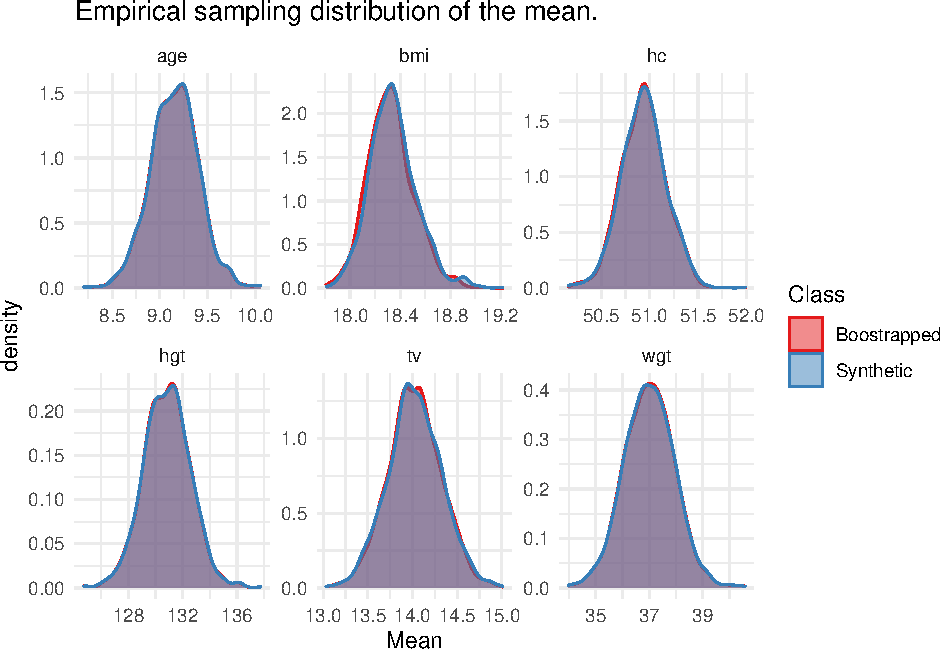
\includegraphics{Manuscript_files/figure-latex/univariate-statistics-1.pdf}
\caption{Empirical sampling distribution of the bootstrapped and
synthetic means of the continuous variables in the boys data.}
\end{figure}

\begin{figure}
\centering
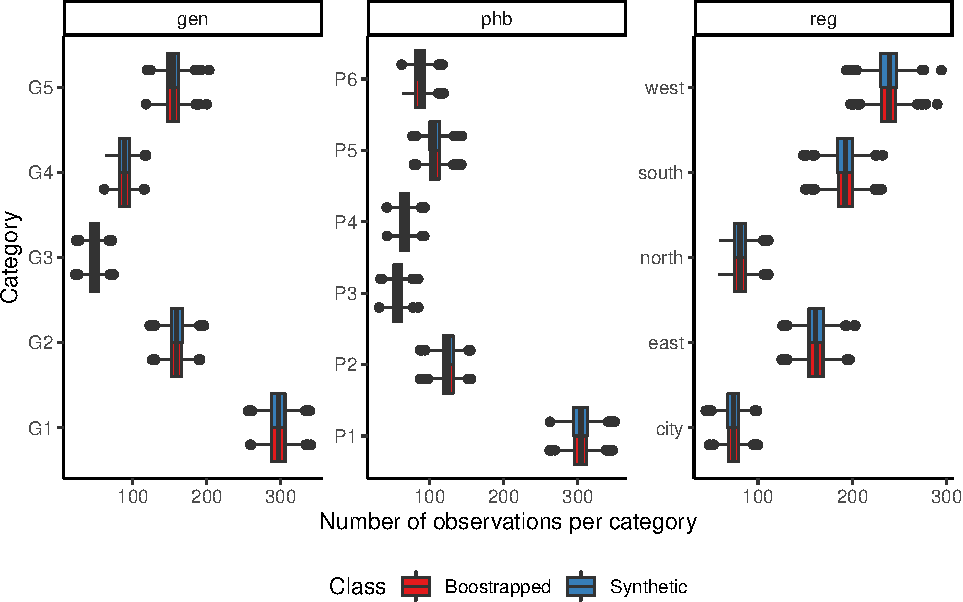
\includegraphics{Manuscript_files/figure-latex/univariate-statistics-II-1.pdf}
\caption{Empirical sampling distribution of the number of observations
within each category of the categorical variables in the bootstrapped
and synthetic boys data.}
\end{figure}

\begin{table}[ht]
\caption{Univariate descriptives for the true data and $m=5$ pooled univariate descriptives for the synthetic data over 1000 simulations. Variable names followed by an asterix ($^*$) are categorical.}
\centering
\begin{tabular}{rrrrrrrrr}
  \hline
 & n & mean & sd & median & min & max & skew & kurtosis \\ 
  \hline
original age & 748 & 9.16 & 6.89 & 10.50 & 0.04 & 21.18 & -0.03 & -1.56 \\ 
  synthetic age & 748 & 9.15 & 6.89 & 10.49 & 0.04 & 20.96 & -0.03 & -1.55 \\ 
  original hgt & 748 & 131.10 & 46.52 & 145.75 & 50.00 & 198.00 & -0.30 & -1.47 \\ 
  synthetic hgt & 748 & 131.06 & 46.50 & 145.32 & 50.69 & 197.16 & -0.30 & -1.47 \\ 
  original wgt & 748 & 37.12 & 26.03 & 34.55 & 3.14 & 117.40 & 0.38 & -1.03 \\ 
  synthetic wgt & 748 & 37.09 & 26.00 & 34.44 & 3.35 & 112.26 & 0.38 & -1.03 \\ 
  original bmi & 748 & 18.04 & 3.04 & 17.45 & 11.73 & 31.74 & 1.14 & 1.79 \\ 
  synthetic bmi & 748 & 18.05 & 3.08 & 17.48 & 11.49 & 32.37 & 1.11 & 1.85 \\ 
  original hc & 748 & 51.62 & 5.86 & 53.10 & 33.70 & 65.00 & -0.91 & 0.12 \\ 
  synthetic hc & 748 & 51.61 & 5.86 & 53.18 & 34.38 & 62.85 & -0.91 & 0.12 \\ 
  original gen* & 748 & 2.53 & 1.59 & 2.00 & 1.00 & 5.00 & 0.52 & -1.36 \\ 
  synthetic gen* & 748 & 2.53 & 1.59 & 2.00 & 1.00 & 5.00 & 0.52 & -1.35 \\ 
  original phb* & 748 & 2.75 & 1.86 & 2.00 & 1.00 & 6.00 & 0.56 & -1.25 \\ 
  synthetic phb* & 748 & 2.75 & 1.86 & 2.00 & 1.00 & 6.00 & 0.56 & -1.24 \\ 
  original tv & 748 & 8.43 & 8.12 & 3.00 & 1.00 & 25.00 & 0.85 & -0.78 \\ 
  synthetic tv & 748 & 8.42 & 8.11 & 3.19 & 1.00 & 25.00 & 0.85 & -0.77 \\ 
  original reg* & 748 & 3.02 & 1.14 & 3.00 & 1.00 & 5.00 & -0.08 & -0.77 \\ 
  synthetic reg* & 748 & 3.02 & 1.14 & 3.00 & 1.00 & 5.00 & -0.08 & -0.76 \\ 
   \hline
\end{tabular}
\end{table}

\hypertarget{bivariate-estimates}{%
\subsection{Bivariate estimates}\label{bivariate-estimates}}

An often used bivariate statistic is Pearson's correlation coefficient.
When evaluating this correlation coefficient on the numeric columns in
the \texttt{boys} data set, the differences between the correlations in
the synthetic and bootstrapped data are very small. These results are
displayed in Table 3.

\begin{table}[H]
\caption{Bivariate correlations of the numerical columns in the true data with in parentheses the corresponding bias of the $m=5$ pooled synthetic correlations over 1000 simulations. All estimates are rounded to 3 decimal places. }
\centering
\begin{tabular}{rcccccc}
  \hline
 & age & hgt & wgt & bmi & hc & tv \\ 
  \hline
age & 1 & 0.976 (0.001) & 0.950 (0.000) & 0.627 (0.009) & 0.853 (0.000) & 0.810 (0.002) \\ 
  hgt & 0.976 (0.001) & 1 & 0.944 (0.001) & 0.596 (0.013) & 0.907 (0.000) & 0.754 (0.000) \\ 
  wgt & 0.950 (0.000) & 0.944 (0.001) & 1 & 0.791 (0.009) & 0.834 (0.000) & 0.817 (0.000) \\ 
  bmi & 0.627 (0.009) & 0.596 (0.013) & 0.791 (0.009) & 1 & 0.588 (0.009) & 0.610 (0.007) \\ 
  hc & 0.853 (0.000) & 0.907 (0.000) & 0.834 (0.000) & 0.588 (0.009) & 1 & 0.623 (0.000) \\ 
  tv & 0.810 (0.002) & 0.754 (0.000) & 0.817 (0.000) & 0.610 (0.007) & 0.623 (0.000) & 1 \\ 
   \hline
\end{tabular}
\end{table}

The correlations obtained from synthetic data are unbiased with respect
to the true data set. The largest bias over 1000 simulations equals
0.013, indicating that the imputation model is capable of preserving the
bivariate relations in the data.

\hypertarget{multivariate-model-inferences}{%
\subsection{Multivariate model
inferences}\label{multivariate-model-inferences}}

First, we evaluate the performance of our synthetic simulation set on a
linear model where \texttt{hgt} is modeled by a continuous predictor
\texttt{age} and an ordered categorical predictor \texttt{phb}. The
results for this simulation can be found in Table 4.

\begin{table}[ht]
\caption{Simulation results for a linear regression model with continuous and ordered categorical predictors. The model evaluated is \texttt{hgt $\sim$ age + phb}. Depicted are the true data estimate and the bias from the true data estimate and the coverage rate of the 95\% confidence interval for the bootstrap and synthetic data sets.}
\centering
\begin{tabular}{rrrrrr}
  \hline
  & & \multicolumn{2}{c}{Bootstrap} & \multicolumn{2}{c}{Synthetic}\\
 term & estimate & bias & cov & bias & cov \\ 
  \hline
(Intercept) & 63.087 & -0.001 & 0.970 & 0.405 & 0.958 \\ 
  age & 7.174 & 0.000 & 0.958 & -0.033 & 0.947 \\ 
  phb.L & -12.250 & 0.008 & 0.950 & 0.582 & 0.927 \\ 
  phb.Q & -1.376 & -0.022 & 0.926 & 0.112 & 0.934 \\ 
  phb.C & -3.564 & 0.051 & 0.915 & 0.301 & 0.912 \\ 
  phb\verb|^|4 & -0.431 & 0.016 & 0.930 & 0.106 & 0.940 \\ 
  phb\verb|^|5 & 2.064 & 0.060 & 0.941 & 0.077 & 0.943 \\ 
   \hline
\end{tabular}
\end{table}

We see that the finite nature of the true data set together with the
design-based simulation setup yields slight undercoverage for the dummy
variables of \texttt{phb}. This finding is observed in both the
bootstrap coverages (i.e.~the fraction of 95\% confidence intervals that
cover the true data parameters) and the synthetic data coverages. Hence,
it is likely that this undercoverage stems from the simulation setup,
rather than the imputation procedure. Besides the undercoverage, there
is a tiny bit of bias in the estimated coefficients of the variable
\texttt{phb} that occurs in the synthetic estimates, but not in the
observed estimates. Yet, since the bias is relatively small and does not
result in confidence invalidity, it seems fair to assume that the
introduced bias is not that problematic.

Second, we evaluate a proportional odds logistic regression model
wherein ordered categorical column \texttt{gen} is modeled by continuous
predictors \texttt{age} and \texttt{hc}, and categorical predictor
\texttt{reg}. The results for this model evaluation are shown in Table
5.

\begin{table}[H]
\caption{Simulation results for a proportional odds logistic regression model with continuous and ordered categorical predictors. The model evaluated is \texttt{gen $\sim$ age + hc + reg}. Depicted are the true data estimate and the bias from the true data estimate and the coverage rate of the 95\% confidence interval for the bootstrap and synthetic data sets.}
\centering
\begin{tabular}{rrrrrr}
  \hline
 & & \multicolumn{2}{c}{Bootstrap} & \multicolumn{2}{c}{Synthetic}\\
 term & estimate & bias & cov & bias & cov \\ 
  \hline
  age & 0.461 & 0.004 & 0.942 & 0.002 & 0.939 \\
  hc & -0.188 & -0.000 & 0.929 & -0.004 & 0.945 \\
  regeast & -0.339 & 0.012 & 0.960 & 0.092 & 0.957\\
  regwest & 0.486 & 0.009 & 0.952 & -0.122 & 0.944\\
  regsouth & 0.646 & 0.012 & 0.966 & -0.152 & 0.943 \\
  regcity & -0.069 & 0.012 & 0.940 & 0.001 & 0.972 \\
  G1$|$G2 & -6.322 & 0.032 & 0.934 & -0.254 & 0.946 \\
  G2$|$G3 & -4.501 & 0.052 & 0.936 & -0.246 & 0.945 \\
  G3$|$G4 & -3.842 & 0.058 & 0.937 & -0.244 & 0.948 \\
  G4$|$G5 & -2.639 & 0.064 & 0.936 & -0.253 & 0.947 \\
   \hline
\end{tabular}
\end{table}

These results demonstrate that the synthetic data analysis yields
inferences that are on par with inferences from the analyses directly on
the bootstrapped datasets. Hence, for the regression coefficients as
well as the intercepts, the analyses on the synthetic data yield valid
results. Nevertheless, a small amount of bias is introduced in the
estimated intercepts of the synthetic data. However, the corresponding
confidence interval coverage rates are actually somewhat higher than the
confidence interval coverage rates of the bootstrapped data. Therefore,
the corresponding inferences do not seem to be affected by this small
bias.

\hypertarget{data-discrimination}{%
\subsection{Data discrimination}\label{data-discrimination}}

When we combine the original and synthetic data, can we predict which
rows come from the synthetic data set? If so, then our synthetic data
procedure would be redundant, since the synthetic set differs from the
observed set. To evaluate whether we can distinguish between the true
data and the synthetic data, we combine the rows from each simulation
synthetic data set with the rows from the true data. We then run a
logistic regression model to predict group membership: i.e.~does a row
belong to the true data or synthetic data. As predictors we take all
columns in the data. The pooled parameter estimates over all simulations
can be found in Table 6.

\begin{table}[H]
\caption{Simulation results for a logistic regression model aimed at discriminating between synthetic records and true records.}
\centering
\begin{tabular}{rrrrrr}
  \hline
 term & estimate & std.error & statistic & df & p.value \\
  \hline
  (Intercept) & 0.22 & 1.15 & 0.19 & 521.93 & 0.60 \\ 
  wgt & 0.00 & 0.02 & 0.25 & 420.19 & 0.60 \\
  hgt & -0.00 & 0.01 & -0.18 & 359.73 & 0.60 \\
  age & -0.00 & 0.05 & -0.00 & 345.73 & 0.62 \\ 
  hc & 0.00 & 0.03 & 0.11 & 415.44 & 0.61\\
  gen.L & -0.00 & 0.42 & -0.00 & 164.76 & 0.65 \\
  gen.Q & -0.01 & 0.21 & -0.04 & 203.38 & 0.63 \\
  gen.C & -0.00 & 0.16 & -0.02 & 239.63 & 0.64 \\
  gen\verb|^|4 & 0.01 & 0.21 & 0.01 & 237.41 & 0.63 \\
  phb.L & -0.02 & 0.44 & -0.04 & 156.54 & 0.64 \\
  phb.Q & -0.01 & 0.22 & -0.02 & 198.20 & 0.64 \\
  phb.C & 0.00 & 0.18 & 0.00 & 211.17 & 0.62 \\
  phb\verb|^|4 & 0.00 & 0.18 & 0.02 & 228.51 & 0.64\\
  phb\verb|^|5 & 0.00 & 0.20 & 0.02 & 248.57 & 0.63\\
  tv & 0.00 & 0.02 & 0.01 & 264.26 & 0.63\\
  regeast & -0.00 & 0.23 & 0.01 & 210.90 & 0.64 \\ 
  regwest & -0.00 & 0.22 & -0.00 & 221.14 & 0.63 \\ 
  regsouth & -0.01 & 0.22 & -0.02 & 226.10 & 0.64 \\ 
  regcity & 0.01 & 0.27 & 0.03 & 204.15 & 0.64 \\ 
  bmi & -0.02 & 0.06 & -0.26 & 320.18 & 0.61 \\
   \hline
\end{tabular}
\end{table}

From these pooled results we can see that the effects for all predictors
are close to zero and non-significant. When we take the predicted values
from the simulated models and compare them with the \emph{real} values,
we obtain the summary statistics in Table 7.

\begin{table}[H]
\caption{Confusion statistics for a prediction model aimed at discriminating between synthetic records and true records.}
\centering
\begin{tabular}{rr}
  \hline
& estimate\\
  \hline
 Accuracy & 0.50381 \\
 Balanced Accuracy & 0.50381 \\
 Kappa & 0.00762 \\
 McnemarPValue & 0.63187 \\
 Sensitivity & 0.50368 \\
 Specificity & 0.50394 \\
 Prevalence & 0.50000 \\
   \hline
\end{tabular}
\end{table}

The accuracy of the predictive modeling effort is not better than random
selection and the Kappa coefficient indicates that a perfect prediction
model is far from realized. The accuracy is quite balanced as there is
no skewness over sensitivity and specificity. These findings indicate
that the synthetic data is indistinguishable from the true data.

\hypertarget{discussion}{%
\section{Discussion}\label{discussion}}

We demonstrate that generating synthetic data sets with \texttt{mice}
using CART in \texttt{R} is a straightforward process that fits well in
a data analysis pipeline. The approach is hardly different from using
multiple imputation to solve problems related to missing data, and hence
can be expected to be familiar to applied researchers. The multiple
synthetic sets yield valid inferences on the true underlying data
generating mechanism, thereby capturing the nature of the original data.
This makes the multiple synthetisation procedure with \texttt{mice}
suitable for further dissemination of synthetic data sets. It is
important to note that in our simulations we used a single iteration and
relied on CART as the imputation method. A single iteration is
sufficient only when the true data is completely observed, or when the
missingness pattern is monotone \citep{drechsler_synthetic_2011}. If
both observed and unobserved values are to be synthesized, then more
iterations and a careful investigation into the convergence of the
algorithm are in order. Synthetic data generation is therein no
different than multiple imputation.

When creating synthetic data with \texttt{mice}, close attention should
be paid to three distinct factors: (i) the additional uncertainty that
is due to synthesizing (part of) the data should be incorporated, (ii)
potential disclosure risks that remain after synthesizing the data
should be assessed, and (iii) the utility of the synthetic data should
be examined. First, the procedure of generating multiple synthetic sets
may seem overly complicated. We would like to emphasize that analyzing a
single synthesized set, while perhaps unbiased, would underestimate the
variance properties that are so important in drawing statistical
inferences from finite data sets. After all, we are often not interested
in the sample at hand, but aim to make inferences about the underlying
data generating mechanism as reflected in the population. Properly
capturing the uncertainty of synthetic data sets, just like with
incomplete data sets, is therefore paramount. To achieve this, we
adopted a bootstrap scheme in our simulations, to represent sampling
from a superpopulation. However, when a single sample should be the
reference, in the sense that the sample reflects the population one
wishes to make inferences about, adjusted pooling rules are required
that are similar to the procedure outlined in \citet{vink2014pooling}.
The corresponding pooling rules have not been derived yet and the
incorporation in data analysis workflows would require proper attention
from developers alike.

Second, it is important that imputers pay close attention to disclosure
risks that remain after creating synthetic data sets. Creating synthetic
data, unless generated from a completely parametric distribution, does
not remove all potential disclosure risks. For example, if the values
that ought to be replaced get the exact same value imputed, the
synthetisation procedure has no use. Additionally, if not all variables
in the data are synthesized, but the variables that are synthesized can
be linked to open access data, a disclosure risk may remain
\citep{drechsler2011empirical}. If the open access data allows for
identification, and the corresponding observations in the synthetic data
can be identified, the variables that are not synthesized may provide
information that should not have been disseminated. The associated
problems generally decrease when the sensitive variables are synthesized
as well. Still, it is important to remain critical regarding the extent
to which the synthetic data might be disclosive. The practical
development of easy to use software to identify which observations are
at risk of disclosure is an area of future work that can improve these
issues. Subsequently, the implementation of ways to overcome such
problems once detected, for example by record swapping as suggested by
\citet{jiang2021balancing}, is welcomed.

Third, the utility of the synthetic data should receive considerable
scrutiny. After all, synthetic data is generated to allow third parties
without access to the data to draw valid inferences. If the quality of
the synthetic data is very poor, the validity of inferences is at stake.
We showed that CART proved to be an adequate method for the data at
hand. However, it may well be that for some problems, using CART for
imputation is not the optimal strategy. We already demonstrated that
imputing deterministic relationships should not be based on CART.
However, due to the variety in possible imputation methods that have
proved to perform well in varying circumstances, providing a single
solution to all synthesis problems seems impossible. If required,
imputers could build up their synthesis models in complexity.
Nevertheless, similarly to past research
\citep[e.g.,][]{burgette_reiter_cart_2010, doove_buuren_recursive_2014, raab_practical_2016},
we showed that CART provides adequate results in general, and therefore
serves as a good starting point.

After imputation, the quality of the synthetic data can be assessed
using various utility measures. The simplest way to assess data quality
is through visual inspection. However, visualizing more than two
dimensions quickly becomes cumbersome, which makes it hard to assess the
accuracy of multivariate relations. Trying to predict whether the data
is observed or synthetic allows to get an intuition of the quality of
the synthesis. This procedure has been advanced by
\citet{snoke2018general}, who proposed a measure of distributional
similarity based on the mean squared error of propensity scores
indicating class belonging for both observed and synthetic data.
Additionally, if one knows the analyses that will be carried out by the
synthetic data users, it is possible to compare the results on the
observed and the synthetic data, allowing to assess the accuracy of the
synthetisation method. Both of these methods have been implemented in
the \texttt{R}-package \texttt{synthpop} \citep{synthpop}, who pioneered
in the field of synthetic data generation in \texttt{R}.

While \texttt{synthpop} is capable to synthesize regardless of missing
data, it is not developed to solve missingness problems. If the data for
synthetisation contains missing values, the missingness will be
considered as a property of the data, and the corresponding synthetic
data sets will contain missing values as well. If the goal is to solve
for the missingness and synthesize the data set, a two-step approach
must be used, in which the missing values are imputed using a different
package, like \texttt{mice}. Subsequently, \texttt{synthpop} can be used
to synthesize the imputed data. Then, given \(m\) multiple imputations
and \(r\) synthetisations, at least \(m \times r\) synthetic data sets
are in order, after which the data can be analysed and the analyses can
be pooled using rules developed by \citet{reiter2004simultaneous}.
However, such an approach would be computationally inefficient and
practically cumbersome, because the architectures of both packages
differ.

The appealing nature of \texttt{mice} therefore lays in its ability to
both solve the missingness problem and create synthetic versions of the
data. Eventually, the flexibility with \texttt{mice} is that unobserved
and observed data values could be synthesized at once, without the need
for a two-step approach. Using \texttt{mice}, \(m\) synthetic sets would
be sufficient. However, as of today, no pooling rules for one-step
imputation of missingness and synthetisation have been developed. The
derivation of those would yield a massive theoretical improvement to
further reduce the burden of creating synthetic data sets.

That said, the fields of synthetic data and multiple imputation are very
much in development. Although efforts have been made to bridge gaps
between these fields, such as in the \texttt{miceadds} package
\citep{miceadds_3.11-6} which links functionality between between
\texttt{synthpop} and \texttt{mice}, further improvements could be made
in that respect. Specifically, \texttt{synthpop} contains a
comprehensive suite of functions that can be used to assess the quality
of synthetic data \citep[e.g., see][]{snoke2018general}, while
\texttt{mice} contains methodology to allow for flexible synthesis of
intricate data structures, such as multilevel data. Being able to use
such functionality interchangeably would greatly benefit data analysts.

The added possibility of synthesizing data with \texttt{mice} in
\texttt{R}, together with the validity of inferences obtained through
this procedure opens up a wealth of possibilities for data dissemination
and further research of initially private data to applied \texttt{R}
users.

% %%%%%%%%%%%%%%%%%%%%%%%%%%%%%%%%%%%%%%%%%%
% %% optional
% \supplementary{The following are available online at www.mdpi.com/link, Figure S1: title, Table S1: title, Video S1: title.}
%
% % Only for the journal Methods and Protocols:
% % If you wish to submit a video article, please do so with any other supplementary material.
% % \supplementary{The following are available at www.mdpi.com/link: Figure S1: title, Table S1: title, Video S1: title. A supporting video article is available at doi: link.}

\vspace{6pt}

%%%%%%%%%%%%%%%%%%%%%%%%%%%%%%%%%%%%%%%%%%
\acknowledgments{We are grateful to Mirthe Hendriks and Stijn van den
Broek for replicating the simulation study on an independent data set.
Additionally, we thank Hanne Oberman, two anonymous reviewers and the
editor for their helpful and insightful comments.}

%%%%%%%%%%%%%%%%%%%%%%%%%%%%%%%%%%%%%%%%%%
\authorcontributions{The authors contributed equally to this work.}

%%%%%%%%%%%%%%%%%%%%%%%%%%%%%%%%%%%%%%%%%%
\conflictsofinterest{The authors declare no conflict of interest.}

%%%%%%%%%%%%%%%%%%%%%%%%%%%%%%%%%%%%%%%%%%
%% optional

\input{"appendix.tex"}

%%%%%%%%%%%%%%%%%%%%%%%%%%%%%%%%%%%%%%%%%%
% Citations and References in Supplementary files are permitted provided that they also appear in the reference list here.

%=====================================
% References, variant A: internal bibliography
%=====================================
%\reftitle{References}
%\begin{thebibliography}{999}
% Reference 1
%\bibitem[Author1(year)]{ref-journal}
%Author1, T. The title of the cited article. {\em Journal Abbreviation} {\bf 2008}, {\em 10}, 142--149.
% Reference 2
%\bibitem[Author2(year)]{ref-book}
%Author2, L. The title of the cited contribution. In {\em The Book Title}; Editor1, F., Editor2, A., Eds.; Publishing House: City, Country, 2007; pp. 32--58.
%\end{thebibliography}

% The following MDPI journals use author-date citation: Arts, Econometrics, Economies, Genealogy, Humanities, IJFS, JRFM, Laws, Religions, Risks, Social Sciences. For those journals, please follow the formatting guidelines on http://www.mdpi.com/authors/references
% To cite two works by the same author: \citeauthor{ref-journal-1a} (\citeyear{ref-journal-1a}, \citeyear{ref-journal-1b}). This produces: Whittaker (1967, 1975)
% To cite two works by the same author with specific pages: \citeauthor{ref-journal-3a} (\citeyear{ref-journal-3a}, p. 328; \citeyear{ref-journal-3b}, p.475). This produces: Wong (1999, p. 328; 2000, p. 475)

%=====================================
% References, variant B: external bibliography
%=====================================
\reftitle{References}
\externalbibliography{yes}
\bibliography{synth.bib}

%%%%%%%%%%%%%%%%%%%%%%%%%%%%%%%%%%%%%%%%%%
%% optional
\sampleavailability{A full simulation archive is available from
\url{https://github.com/amices/Federated_imputation/tree/master/manuscript}.}

%% for journal Sci
%\reviewreports{\\
%Reviewer 1 comments and authors’ response\\
%Reviewer 2 comments and authors’ response\\
%Reviewer 3 comments and authors’ response
%}

%%%%%%%%%%%%%%%%%%%%%%%%%%%%%%%%%%%%%%%%%%
\end{document}
